The calibration layer is responsible for the calibration of the software to a specific user. This data is crucial to obtaining acurate gaze tracking information and displaying it for the user/system.

\begin{figure}[h!]
	\centering
	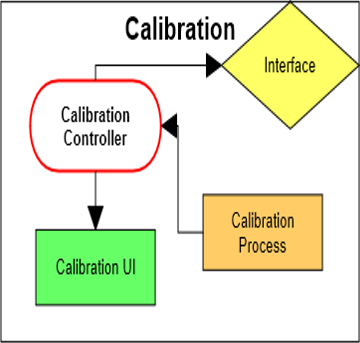
\includegraphics[width=0.60\textwidth]{images/calibration}
	\caption{Example subsystem description diagram}
\end{figure}

\subsection{Calibration UI}
The calibration UI displays information to the user so that that the calibration process can calculate accurate data. This is achieved by moving a dot around on the screen for the user to follow with their eyes.

\subsubsection{Assumptions}
The os of the system the UI is displayed on will be windows 10.

\subsubsection{Responsibilities}
This subsystem must accurately display the dot on the screen at the proper place and for the appropriate amount of time.

\subsubsection{Subsystem Interfaces}

\begin {table}[H]
\caption {Subsystem interfaces} 
\begin{center}
    \begin{tabular}{ | p{1cm} | p{6cm} | p{3cm} | p{3cm} |}
    \hline
    ID & Description & Inputs & Outputs \\ \hline
    \#1 & Controller/UI & \pbox{3cm}{Begin} & \pbox{3cm}{N/A}  \\ \hline
    \end{tabular}
\end{center}
\end{table}

\subsection{Calibration Process}
The calibration process receives camera information via its controller, and information about when the UI subsystem began in order to build accurate calibration information about the user.

\subsubsection{Assumptions}
The UI always performs its task in the alloted time-frame expected by the calibration process.

\subsubsection{Responsibilities}
Build accurate calibration data about the user.

\subsubsection{Subsystem Interfaces}

\begin {table}[H]
\caption {Subsystem interfaces} 
\begin{center}
	\begin{tabular}{ | p{1cm} | p{6cm} | p{3cm} | p{3cm} |}
		\hline
		ID & Description & Inputs & Outputs \\ \hline
		\#1 & Calibration Process/Controller & \pbox{3cm}{Camera Data \\ Begin} & \pbox{3cm}{Calibration File}  \\ \hline
	\end{tabular}
\end{center}
\end{table}

\subsection{Subsystem 3}
The calibration controller is responsible for coordinating the beginning of the calibration process, passing information to the calibration process, and ensuring the delivery of calibration data back to the rest of the system. This model allows the UI or Process to change independently of each other, all while maintaining a seamless interface for the rest of the system.

\subsubsection{Responsibilities}
Begin the calibration process in a timely manner and return accurate calibration data to the rest of the system.

\subsubsection{Subsystem Interfaces}

\begin {table}[H]
\caption {Subsystem interfaces} 
\begin{center}
	\begin{tabular}{ | p{1cm} | p{6cm} | p{3cm} | p{3cm} |}
		\hline
		ID & Description & Inputs & Outputs \\ \hline
		\#1 & Controller/interface & \pbox{3cm}{Device Data \\ Begin} & \pbox{3cm}{Calibration File}  \\ \hline
		\#2 & Controller/UI & \pbox{3cm}{N/A} & \pbox{3cm}{Begin}  \\ \hline
		\#3 & Controller/Process & \pbox{3cm}{Calibration Data} & \pbox{3cm}{Begin \\ Device Data}  \\ \hline
	\end{tabular}
\end{center}
\end{table}

